%%%%%%%%%%%%%%%%%%%%%%%%%%%%%%%%%%%%%%%%%%%%%%%%%%%%%%%%
%%%%%%%%%%%%%%%%%%%%%%%%%%%%%%%%%%%%%%%%%%%%%%%%%%%%%%%%
\newpage
\part{Estructuras de Datos Dinámicas}
\setcounter{section}{0}
%\begin{center}
%\huge{\textbf{Estructuras de Datos Dinámicas}} \\
%\end{center}

Una estructura de datos dinámica se refiere a una organización en memoria como una colección de datos que es flexible al momento de expandirse o reducirse en tamaño en tiempo de ejecución de un algoritmo. En muchas ocasiones, este tipo de estructuras permite al programador tener control sobre cuánta memoria está empleando. Las estructuras dinámicas juegan un papel muy importante en diversos lenguajes de programación ofreciendo la posibilidad de ajustar la cantidad de memoria que un programa empleará.

Las estructuras de datos estáticas es el caso opuesto a las dinámicas, donde el tamaño de la estructura es fija. Son ideales para almacenar un número fijo de elementos pero carecen de la flexibilidad para consumir memoria adicional si la requieren o liberar memoria para mejorar el rendimiento de los programas.

Entonces, para cada tipo de dato se presenta la definición de ésta, una posible clasificación (si es posible), su especificación e implementación. La idea de la especificación empleando una clase está en responder ¿qué hace? la estructura y no en ¿cómo lo hace?. Para responder la segunda pregunta, se utilizará la subsección de Implementación. En este documento se presentan las estructuras básicas dinámicas: tipo List, Stack y Queue.

%%%%%%%%%%%%%%%%%%%%%%%%%%%%%%%%%%%%%%%%%%%%%%%%%%%%%%%%
\section{Tipo List}

El tipo de dato List representa a una lista de elementos la cual permite representar una serie de actividades, tareas, objetos, etc. Una lista del mercado, una lista de cosas por hacer, una lista de libros por leer, entre muchos otros ejemplos de la vida diaria.

Una lista es una colección finita de elementos del mismo tipo, ordenados de acuerdo a su posición en la lista. Podemos utilizar la siguiente notación para denotar una lista $L$ de $n$ elementos: si la lista es vacía se denota como $L=()$, y si contiene elementos entonces como $L=(e_1, e_2, ..., e_k)$. Generalmente las listas tienen las siguientes características:
\begin{itemize}
\item Todos los elementos son de un mismo tipo de dato
\item Las listas pueden crecer o decrecer en tiempo de ejecución
\item Se pueden subdividir en sublistas
\item Su acceso es de forma secuencial (un elemento seguido de otro)
\end{itemize}

Un tipo List es una estructura flexible que puede crecer y acortarse según se requiera. Mediante una posición dentro de la lista es posible moverse y efectuar operaciones básicas como insertar, eliminar, modificar un elemento, o concatenarse con otras listas. Una clasificación básica de listas puede ser de acuerdo al número de enlaces o conexiones con los otros elementos de la lista. Así, se pueden clasificar en listas simplemente enlazadas (acceso en un solo sentido) o doblemente enlazadas (acceso en ambos sentidos). A continuación se describe cada una de ellas.

%%%%%%%%%%%%%%%%%%%%%%%%%%%%%%
\subsection{Simplemente Enlazada}

Los elementos en una lista están colocados en forma secuencial. Ahora, esto no quiere decir que están contiguos en memoria, de hecho, en estructuras dinámicas los elementos se pueden encontrar dispersos en memoria pero enlazados desde una posición y tener acceso al siguiente elemento.

Para una lista simplemente enlazada, se define una estructura (denominada Node) que almacenará el valor como tal de la estructura homogénea (denominada List), y un enlace al próximo elemento desde dicha estructura Node. Primeramente, se realizará la especificación de una lista sin entrar en detalles de su implementación basado en un conjunto de atributos y métodos dentro de una clase. Luego, se muestra las implementaciones posibles dada dicha especificación.

%%%%%%%%%%%%%%%%%%%%%%%%%%%%%%
\subsubsection{Especificación}

En una especificación de una estructura de datos se pueden diferenciar dos roles principales: usuario y programador. En el rol de usuario, se emplea la estructura de datos sin conocer cómo está implementado sino empleando los métodos dispuestos en la especificación de la estructura. Ahora, el rol de programador incluye el uso de la estructura según su especificación y la forma como será implementado (i.e. uso de variables, desarrollo de las unidades invocables).

Para la especificación de la lista, se define como atributo un tipo de dato que represente una posición dentro de una lista. Esta posición en su implementación puede ser un tipo Integer, Pointer, entre otros. Así, el tipo List se especifica en la siguiente clase.

\begin{lstlisting}[upquote=true, language=pseudo]
class List <T>					// definición de una plantilla o template de listas, T indica el tipo de dato
public:
  Type <...> tPosition			// tipo de dato posición para desplazarse (sin mostrar la implementación)

  Constructor List()			// construye la lista vacía ().
  Destructor List()			//destructor de la clase. Libera la lista de memoria

  function IsEmpty() : Boolean		// retorna True si la lista es vacía, y false en caso contrario
  function First() : tPosition		// retorna la posición del 1er elemento de la lista, o Last() si la lista es vacía
  function Last() : tPosition		// retorna la posición final de lista (posición después del último)
  void Next(ref tPosition pValue)	// Pre: pValue != Last().Mueve la posición hacia la posición siguiente de la lista
  function Get (tPosition pValue): ref T// Retorna la referencia a la información contenida en pValue
  void Insert (ref T x, tPosition pValue)// Inserta x antes de la posición pValue
  void Delete (tPosition pValue)	// Pre: pValue!=Last(). Elimina el elemento de pValue. La posición pValue queda						// referenciando a un elemento inexistente
  function Size() : Integer		// retorna el número de elementos en la lista
end
\end{lstlisting}

Nótese que la función Last retorna la posición final o posición disponible al final de la lista, lo cual difiere a ser el último elemento de la lista. Del mismo modo, es importante destacar que existe pase de parámetros por referencia y retorno de la referencia del tipo de dato $T$ que es empleado de forma genérica como plantilla en la clase.

%%%%%%%%%%%%%%%%%%%%%%%%%%%%%%
\subsubsection{Ejemplos}

A continuación una serie de ejemplos donde se utiliza las unidades invocables presentes en el tipo List sin conocer su implementación.

- Dada una lista, imprimir sus elementos
\begin{lstlisting}[upquote=true, language=pseudo]
void PrintList(ref List <T> L)
  tPosition tIndex = L.First()
  while tIndex != L.Last() do
    Print (*L.Get(tIndex))
    L.Next(ref tIndex)
  end
end
\end{lstlisting}

El algoritmo consiste simplemente en dada la primera posición de la lista, iterar de forma secuencial sobre cada elemento e imprimir su valor.

- Dada una lista de enteros, asignar el valor de 666 a todos sus elementos:
\begin{lstlisting}[upquote=true, language=pseudo]
void Change (ref List <Integer> L)
  tPosition tIndex = L.First()
  Const Integer iSixSixSix = 666
  while tIndex != L.Last() do
    L.Insert(ref iSixSixSix, tIndex) 	// también se puede emplear *L.Get(tIndex) = iSixSixSix
    L.Next(ref tIndex)
  end
end
\end{lstlisting}

Siendo muy similar al algoritmo anterior, dado el primer elemento de la lista se itera sobre cada elemento y se emplea la función Insert dada la posición y la constante a añadir.

- Dada una lista de valores enteros, eliminar todos los elementos que tengan valor mayor a 15:
\begin{lstlisting}[upquote=true, language=pseudo]
void Delete15 (ref List <Integer> L)
  tPosition tIndex = L.First()
  while tIndex != L.Last() do
    if *L.Get(tIndex) > 15 then
      tPosition tTemp = tIndex
      L.Next (ref tTemp)
      L.Delete (tIndex)
      tIndex =  tTemp
    else
      L.Next(ref tIndex)
    end
  end
end
\end{lstlisting}

Esta función busca todas las posiciones que cumplen con la condición $> 15$ y para cada una ``salta" una posición más allá de la actual con el fin de eliminar todos aquellos elementos que cumple dicha condición. Existen algunas consideraciones que se deben tomar en cuenta al momento de su ejecución, pero que dependen de la implementación tal como liberación de la memoria si es dinámica, enlace de los elementos de forma correcta, entre otros.

-Concatenar dos listas del tipo User llamadas A y B, y dejar el resultado en la lista A
\begin{lstlisting}[upquote=true, language=pseudo]
void Concat (ref List<User> A, B)
  tPosition tIndex = B.First()
  while tIndex != B.Last() do
    A.Insert(B.Get(tIndex), A.Last())
    B.Next(ref tIndex)
  end
end
\end{lstlisting}

Al igual que operar sobre un par de arreglos, dada la lista A y a partir de su posición final se anexará cada uno de los elementos que pertenecen a B hasta que no queden elementos en B. Nuevamente, aspectos como no eliminar los elementos de B o el tamaño máximo de elementos de A, son concernientes al programador.

%%%%%%%%%%%%%%%%%%%%%%%%%%%%%%
\subsubsection{Implementación}

La forma básica de implementar una lista simplemente enlazada es empleando un arreglo unidimensional dinámico, donde a medida que se agreguen o eliminen elementos, el tamaño de la lista se modifica. Una operación de acceso, inserción, eliminación y búsqueda tendrá complejidad $O(n)$, pero con una implementación simple. Otra forma de implementar el tipo List con arreglos, es empleando un arreglo de registros, donde cada posición contiene el valor a almacenar (información) y el índice al próximo elemento dentro de la lista. Al mismo tiempo, es posible tener sublistas para definir las próximas posiciones libres u ocupadas del arreglo. A diferencia de la implementación anterior, ésta es estática y se debe definir un tamaño máximo de elementos.

En diversos lenguajes de programación existen implementaciones dinámicas de listas como es el caso en C++ empleando la librería STL (i.e. vector), en Java de forma nativa (i.e. Vector), en Python se emplea como un tipo de dato secuencia, entre otros. A continuación, estudiaremos diversas implementaciones . 

\paragraph{Implementación con arreglos}

Para la implementación con arreglos se asume que existe un tamaño máximo o que se modifica de forma dinámica. Ahora, el punto importante es que para cada posición dentro del arreglo se debe conocer cuál es el próximo elemento dada una posición. 

De este modo, la Fig. \ref{fig:listarray} muestra un ejemplo de una posible distribución del tipo List empleando arreglos.

\begin{figure}[htpb!]
  \begin{center}
    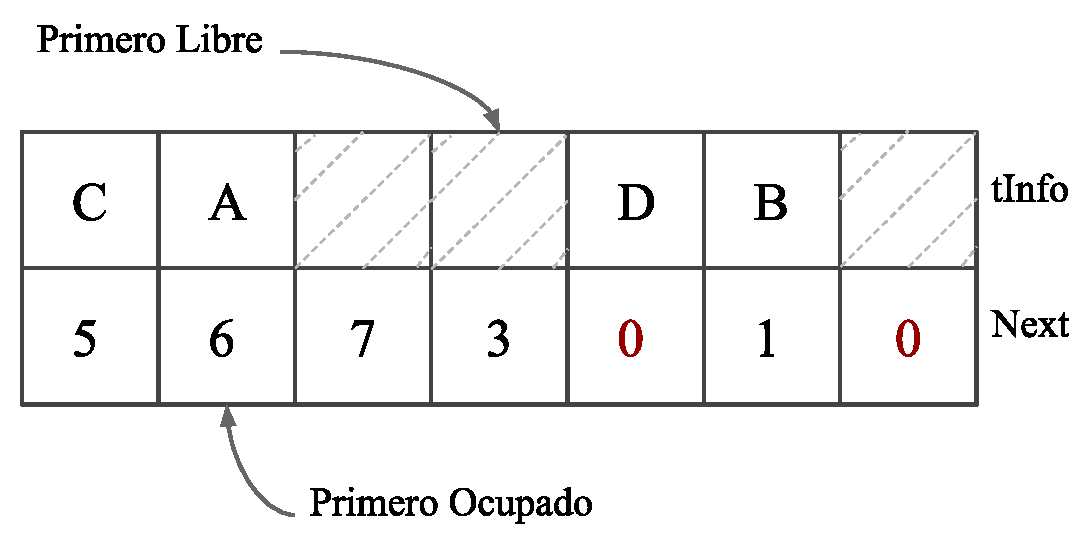
\includegraphics[width=0.5\textwidth]{images/listarray.eps}
  \end{center}
  \caption{Ejemplo de representación de una lista simplemente enlazada empleando arreglos.}
  \label{fig:listarray}
\end{figure}

La Fig. \ref{fig:listarray} es un instante de tiempo en durante la ejecución de la estructura. En esta implementación se consideran dos posiciones claves que son la primera posición libre y la primera posición ocupada. Se debe mantener un arreglo del tipo Position, y otro donde se almacena el tipo de dato de la lista.

En el ejemplo, la primera casilla ocupada está en la posición 2 correspondiente al valor (tInfo)  'A'. Desde allí, el próximo campo ocupado (Next) se encuentra en el valor que indica el arreglo de ocupados, es decir, la posición 6. La posición 6 corresponde al valor 'B'., luego a la posición 1 para el valor 'C', y finalmente el último valor está en la posición 5 correspondiente a 'D'. El próximo elemento ocupado desde 'D' corresponde al valor de 0, este valor indica la finalización de la lista.

De forma similar ocurre con la primera posición libre en la posición 4, la segunda libre será la posición 3, luego la posición 7 y ésta será la última para dicho arreglo.

\paragraph{Implementación con apuntadores}

En este caso, tenemos un conjunto de nodos enlazados mediante el campo denominado pNext. Por otro lado, la lista contendrá a un apuntador al primer elemento de dicha lista y el valor pNext del último nodo apunta a NIL. En esta versión las operaciones de Insertar y Eliminar son de complejidad $O(n)$.

En la Fig. \ref{fig:listas} se muestra de forma visual la representación de una lista simplemente enlazada. Se nota que el inicio de la lista está indicada por el apuntador $pFirst$, de allí el nodo con $tInfo = e_1$ indica el siguiente elemento de la lista a través del campo $pNext$ hasta llegar al final de la lista. Empleando apuntadores, el final de la lista se ubica cuando el próximo es NIL (representado por el símbolo $\backslash \backslash$ en la figura.

\begin{figure}[!htpb]
\centering
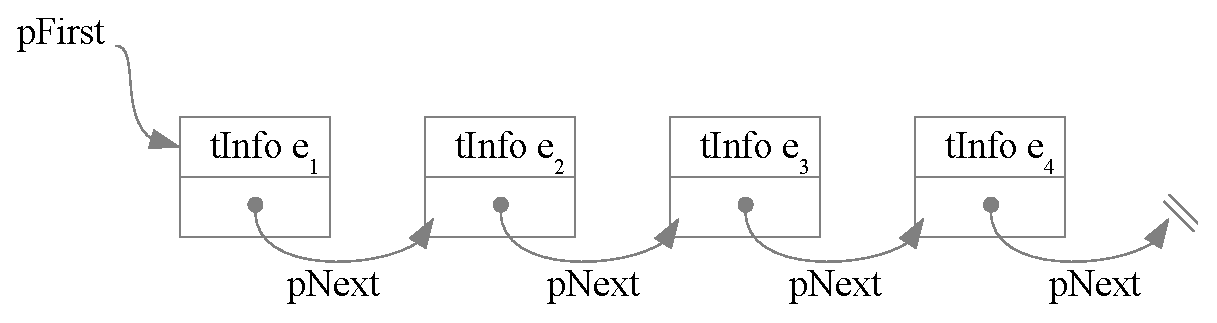
\includegraphics[scale=.7]{images/listas.eps}
\caption{Representación visual de una estructura de lista simplemente enlazada empleando apuntadores.}
\label{fig:listas}
\end{figure}

\begin{lstlisting}[upquote=true, language=pseudo]
class Node <T>
public:
  T tInfo
  Node<T>* pNext
end

class List <T>
private:
  Node<T>* pFirst		// apuntador al primer nodo 
  Integer iN				// número de elementos en la lista 

public:
  Type Node<T>* tPosition		// la posición es un apuntador a Node*<T>

  Constructor List () 
    iN = 0
    pFirst = NIL
  end

  Destructor List ()
    Node<T>* pTemp
    while pFirst != NIL then
      pTemp = pFirst
      pFirst = (*pFirst).pNext
      delete pTemp
    end
  end

  function IsEmpty() : Boolean
    return pFirst == NIL
  end

  function First() : tPosition
    return pFirst
  end

  function Last() : tPosition
    return NIL
  end

  void Next(ref tPosition pValue)
    pValue = *pValue.pNext
  end

  function Get(tPosition pValue) : ref T
	return ref (*pValue).tInfo
  end

  void Insert(ref T x, tPosition pValue) 	//O(n). Se require que el nodo anterior apunte al próximo nodo 
    Node<T>* pNew = new Node
    (*pNew).tInfo = *x
    (*pNew).pNext = pValue
    if (pFirst == NIL or pFirst == pValue) then
      pFirst = pNew
    else
      Node<T>* pTemp = pFirst
      while *pTemp.pNext != pValue do
        pTemp = *pTemp.pNext
      end
     *pTemp.pNext = pNew
    end
    iN = iN + 1
  end

  void Delete(tPosition pValue)
    if pFirst == pValue then
      pFirst = *pFirst.pNext
    else
      Node<T>* pTemp = pFirst
      while *pTemp.pNext != pValue do
        pTemp = *pTemp.pNext
      end
      *pTemp.pNext = *pValue.pNext
    end
    delete pValue
    iN = iN - 1
  end

  function Size() : Integer
    return iN
  end
end
\end{lstlisting}

Es posible lograr la operación de inserción y eliminación de complejidad O(1) si se cuenta con un puntero al nodo anterior. Del mismo modo, si se contará con un puntero a los nodos anteriores es posible hacer el recorrido en ambos sentidos (ver sección \ref{lb:dobleenlazada}.

\paragraph{Implementación con apuntadores y nodo cabeza}

Un nodo cabeza es un nodo especial por donde se realizarán las operaciones de la lista. Con el nodo cabeza se garantiza que todo nodo tiene un predecesor en la lista, y la posición de un nodo se referenciará desde la posición del nodo anterior. En esta implementación, todas las operaciones son de complejidad $O(1)$. Adicionalmente, como atributo de la clase se requiere mantener un apuntador al último nodo para que la operación Last() sea de complejidad $O(1)$.
\begin{lstlisting}[upquote=true, language=pseudo]
class Node <T>
public:
  T tInfo
  Node<T>* pNext
end

class List <T>
private:
  Node<T>* pFirst				// apuntador al nodo cabeza. Este apuntador no se modifica
  Node<T>* pLast				// apuntador al último nodo (nodo cuyo próximo es NIL)
  Integer iN					// número de elementos en la lista 

public:
  Type Node<T>* tPosition		// la posición es un apuntador a Node*<T>

  Constructor List () 
    iN = 0
    pFirst = new Node ()
    pLast = pFirst
    *pFirst.pNext = NIL
  end

  Destructor List ()
    Node<T>* pTemp
    while pFirst != NIL then
      pTemp = pFirst
      pFirst = (*pFirst).pNext
      delete pTemp
    end
  end

  function IsEmpty() : Boolean
    return *pFirst.pNext == NIL
  end

  function First() : tPosition
    return pFirst
  end

  function Last() : tPosition
    return pLast
  end

  void Next(ref tPosition pValue)
    pValue = *pValue.pNext
  end

  function Get(tPosition pValue) : ref T
    return ref *(*pValue.pNext).tInfo
  end

  void Insert(ref T x, tPosition pValue)
    Node<T>* pNew = new Node
    (*pNew).tInfo = *x
    if (pFirst == pValue) then // insertando de primero
      *pNew.pNext = *pFirst.pNext
      *pFirst.pNext = pNew
    else
      *pNew.pNext = *pValue.pNext 
      *pValue.pNext = pNew
    end
    if pLast == pValue then
      pLast = pNew
    end
    iN = iN + 1
  end

  void Delete (tPosition pValue)
    if (*pValue.pNext == pLast) then 
      pLast = pValue 
    end
    Node<T>* pTemp = *pValue.pNext
    *pValue.pNext = (*(*pValue.pNext)).pNext 
    delete pTemp
    N = N-1; 
  end

  function Size() : Integer
    return iN
  end
end
\end{lstlisting}

\paragraph{Implementación eficiente con apuntadores}

En la primera implementación con apuntadores todas las operaciones son $O(1)$ a excepción de las funciones Insert y Delete. Para lograr que estas operaciones sean $O(1)$, se debe emplear como posición la dirección del campo pNext del nodo anterior. Dado que el primer nodo no posee un nodo anterior, se emplea la dirección de pFirst. De esta manera, no se buscará al nodo anterior en la inserción y eliminación ya que se referenciará al campo pNext del nodo anterior. Así, todas las operaciones son $O(1)$ a excepción de Last() porque ésta debe retornar el apuntador al campo pNext del último nodo (o la dirección de pFirst) de complejidad $O(N)$ en el peor de los casos. Para evitar ello, se introduce un atributo apuntador para el último campo pNext como atributo de la lista, el cual posiblemente deba actualizarse durante la operación de inserción y eliminación.
\begin{lstlisting}[upquote=true, language=pseudo]
class Node <T>
public:
  T tInfo
  Node<T>* pNext
end

class List <T>
public:
  Type Node<T>** tPosition		// la posición es un apuntador doble a Node**<T>

private:
  Node<T>* pFirst				// apuntador al primer nodo 
  tPosition pLast			// apuntador al último nodo
  Integer iN				// número de elementos en la lista 

public:
  Constructor List () 
    iN = 0
    pFirst = NIL
    pLast = ref pFirst
  end

  Destructor List ()
    Node<T>* pTemp
    while pFirst != NIL then
      pTemp = pFirst
      pFirst = (*pFirst).pNext
      delete pTemp
    end
  end

  function IsEmpty() : Boolean
    return pFirst == NIL
  end

  function First() : tPosition
    return ref pFirst
  end

  function Last() : tPosition
    return pLast
  end

  void Next(ref tPosition pValue)
    pValue = ref (*(*pValue.pNext))
  end

  function Get(tPosition pValue) : ref T
    return ref (*(*pValue)).tInfo
  end

  void Insert(ref T x, tPosition pValue)
    Node<T>* pNew = new Node
    (*pNew).tInfo = *x
    if pFirst == NIL then 		// la lista estaba vacía
      *pNew.pNext = NIL
      pFirst = pNew
      pLast = ref *pNew.pNext
    elseif (*pValue == pFirst) then	// insertando en la lista de primero
      *pNew.pNext = pFirst
      pFirst = pNew
    elseif *pValue == NIL then	// insertando en la lista de último
      *pLast = pNew
      *pNew.pNext = NIL
      pLast = ref (*pNew).pNext
    else				// insertando en un nodo intermedio
      *pNew.pNext = *pValue
      *pValue = pNew
    end
    iN = iN + 1
  end

  void Delete (tPosition pValue) 
    Node<T>* pTemp = *pValue
    if *pValue == pFirst then 	// se elimina el primer elemento 
      pFirst = *pFirst.pNext
      if pFirst == NIL then
        pLast = ref pFirst
      end
    elseif ((*(*pValue)).pNext == NIL) then //se elimina el ultimo element
      pLast = pValue
      *pValue = NIL
    else				// se elimina un nodo intermedio
    *pValue = (*(*pValue)).pNext
    end
    delete pTemp
    iN = iN-1
  end

  function Size() : Integer
    return iN
  end
end

\end{lstlisting}

%%%%%%%%%%%%%%%%%%%%%%%%%%%%%%
\subsection{Doblemente Enlazada} \label{lb:dobleenlazada}

La idea central de una lista doblemente enlazada es mantener una relación de conectividad de cada elemento de la lista con el elemento próximo y anterior. Entonces, es posible recorrer la lista en ambos sentidos: desde el inicio al final, y del final al inicio. Para ello se requiere de una marca de finalización para cada recorrido. Para dicha marca se emplea una función denominada End que sirve como parada cuando se recorre desde el inicio al final, y otra función llamada Start que es cuando se recorre en sentido inverso. Del mismo modo, se permiten las operaciones de PreInsert y PostInsert debido a que será posible insertar antes y después de una posición dada.

%%%%%%%%%%%%%%%%%%%%%%%%%%%%%%
\subsubsection{Especificación}

La especificación de las operaciones de una lista doblemente enlazada general se puede definir como una clase de la siguiente forma:

\begin{lstlisting}[upquote=true, language=pseudo]
class ListDouble <T>
public:
    Type <...> tPosition			// tipo de dato posición para desplazarse (no se muestra la implementación)

    Constructor ListDouble ()		// construye la lista vacía ()
    Constructor ListDouble (ref List <T> lSource)  // constructor de copia
    Destructor ListDouble ()		// destructor de la clase. Libera lavlc lista de memoria

    function IsEmpty() : Boolean		// retorna True si la lista es vacía, y false en caso contrario
    function Start() : tPosition		// retorna la posición del inicio de la lista (previo al primero)
    function First() : tPosition		// retorna la posición del 1er elemento de la lista
    function End() : tPosition		// retorna la posición final de la lista (después del último) 
    function Last() : tPosition		// retorna la posición del último elemento de la lista
    void Next(ref tPosition pValue)	// Pre: pValue!= End()
    void Prev(ref tPosition pValue)	// Pre: pValue!= Start()
    function Get (tPosition pValue): ref T// Retorna la referencia a la información contenida en pValue
    void PreInsert (ref T x, tPosition pValue)// Pre: pValue!= Start().Inserta x antes de  pValue. 
    void PostInsert (ref T x, tPosition pValue)// Pre: pValue!= End().Inserta x después de pValue. 
    void Delete (tPosition pValue)	// Pre: pValue es válida. Elimina el elemento de posición pValue.
    function Size() : Integer		// retorna el número de elementos en la lista
end
\end{lstlisting}

%%%%%%%%%%%%%%%%%%%%%%%%%%%%%%
\subsubsection{Ejemplos}

Una serie de ejemplos del uso de la especificación de la clase ListDouble.

- Imprimir los elementos de una lista en orden inverso 
\begin{lstlisting}[upquote=true, language=pseudo]
void PrintList(ref ListDouble <Integer> L) 
    tPosition tIndex = L.Last()
    while (tIndex != L.Start()) do
        Print (*L.Get(tIndex)) 
        L.Prev (ref tIndex) 
    end 
end
\end{lstlisting}

En este algoritmo se comienza desde la posición del último elemento (Last) y se itera con la función Prev hasta llegar a Start. Es importante destacar que la condición de parada es Start y no First (First representa al 1er elemento de la lista).

- Eliminar los últimos 3 elementos de la lista de enteros
\begin{lstlisting}[upquote=true, language=pseudo]
void Delete3(ref ListDouble <Integer> L) 
    tPosition tIndex = L.Last(), tTemp
    Integer iCont = 0 
    while (tIndex != L.Start() and iCont  != 3) do
        tTemp = tIndex 
        L.Prev(ref tTemp)
        L.Delete(tIndex) 
        tIndex = tTemp 
        iCont = iCont + 1
    end
end
\end{lstlisting}

Nuevamente, empezando desde la última posición y hasta llegar al inicio, se cuentan 3 elementos y son eliminados de la lista doblemente enlazada.

%%%%%%%%%%%%%%%%%%%%%%%%%%%%%%
\subsubsection{Implementación}

De forma similar que las listas simplemente enlazadas, existen diversas implementaciones de las listas doblemente enlazadas: empleando arreglos y apuntadores. Un aspecto relevante es la posibilidad de particularizar la estructura de datos para resolver problemas específicos. Por ejemplo, buscar en un rango ordenado de valores de forma eficiente un valor; representar los lugares de una mesa redonda como una lista circular (caso particular de lista doblemente enlazada); o emplear múltiples apuntadores dentro de una lista para crear sub-listas (una lista de enteros donde se ordenen los números pares e impares como sublistas de ésta).

En la Fig. \ref{fig:listas2} se muestra una representación de una estructura ListDouble empleando apuntadores. En ella, existen dos apuntadores principales pFirst y pLast. Al mismo tiempo, en cada nodo existen 2 apuntadores que van a permitir el recorrido en ambos sentidos: pNext y pPrev.

\begin{figure}[!htb]
\centering
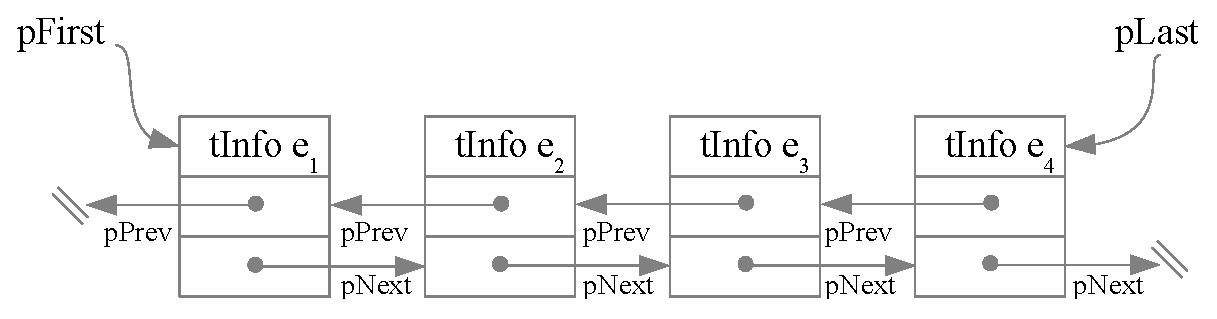
\includegraphics[scale=.7]{images/listas2.eps}
\caption{Representación visual de una estructura de lista simplemente enlazada empleando apuntadores.}
\label{fig:listas2}
\end{figure}

Es posible que una lista con enlaces no solo tenga una conexión con el nodo anterior y con el previo, sino que requiera conectarse con otro nodo de forma ``salteada" de acuerdo ala naturaleza del problema. Por ello, a continuación se muestra las listas multienlazadas o con múltiples enlaces.

%%%%%%%%%%%%%%%%%%%%%%%%%%%%%%%%%%%%%%%%%%%%%%%%%%%%%%%%
\section{Lista Multienlazada}

Una lista multienlazada o n-enlazada tiene como característica que sus nodos contienen enlaces que los asocian con más de una lista. Esto quiere decir que con una misma lista física, los diferentes apuntadores hacen que en realidad se enlacen $n$ listas lógicas o se manipulen de forma particular de acuerdo a dichos enlaces.

De este modo, las listas doblemente enlazadas son un caso particular de listas multienlazadas donde:
\begin{enumerate}
\item Cada nodo tiene 2 identificadores de tipo Pointer
\item Los apuntadores son exactamente inversos una de otro
\end{enumerate}

Así, en una lista multienlazada cada nodo puede tener cualquier cantidad de apuntadores a otros nodos que pueden formar diversas estructuras o no. Por ejemplo, dada una lista de personas enlazada entre sí de dos maneras:
\begin{enumerate}
\item Ordenada alfabéticamente por el primer apellido
\item Ordenada ascendentemente por su documento de identidad
\end{enumerate}

Es posible representar dicha información como dos listas, pero existe el problema de la doble representación de los nodos (nodos duplicados) tanto en su representación como en el desarrollo de sus operaciones. Entonces, las operaciones de Insert o Delete deben realizarse en ambas listas. Una solución es representar mediante el uso de apuntadores en una lista multienlazada estas dos listas lógicas en una sola lista física, definiendo sus nodos (ver Fig. \ref{fig:multifirst}).
 
\begin{figure}[htp!]
  \begin{center}
    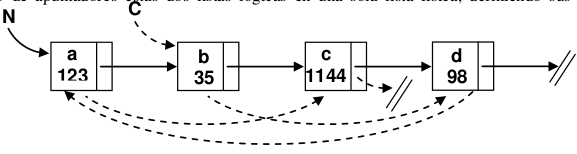
\includegraphics[width=0.75\textwidth]{images/first.png}
  \end{center}
  \caption{Ejemplo de dos listas lógicas en una sola lista multienlazada.}
  \label{fig:multifirst}
\end{figure}
 
 El puntero $N$ y las flechas continuas representan la lista ordenada por nombre y el puntero $C$ y las flechas punteadas la lista ordenada por documento de identidad. También esta lista se puede representar con el uso de un nodo cabeza. Dicho nodo cabeza contedrá un puntero al nodo inicial que representa el comienzo de cada lista lógica, tal como se muestra en la Fig. \ref{fig:multisecond}.

\begin{figure}[htp!]
  \begin{center}
    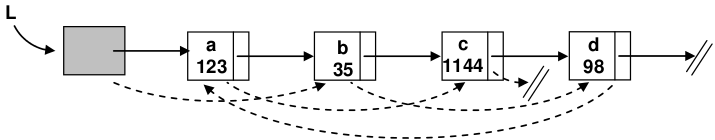
\includegraphics[width=0.75\textwidth]{images/second.png}
  \end{center}
  \caption{Ejemplo de dos listas lógicas en una sola lista multienlazada con nodo cabeza L.}
  \label{fig:multisecond}
\end{figure}


Las estructuras de datos de la lista multienlazada para el ejemplo anterior se pueden definir como:

\begin{lstlisting}[upquote=true, language=pseudo]
class CPerson
public:
  String strName
  Integer iDocIdentidad
end

class Node
public:
  CPerson Info
  Node* pNextN
  Node* pNextC
end
\end{lstlisting}

En el caso de emplear dos apuntadores para cada lista, la definición queda como:

\begin{lstlisting}[upquote=true, language=pseudo]
class ListPerson
public:
  Node* N	//primer elemento de la lista de nombres
  Node* C	//primer elementos de la lista de documentos de identidad
end
\end{lstlisting}

Y en caso de emplear nodo cabeza, solo cambia la definición de ListPerson y se agrega la estructura NodeHead.

\begin{lstlisting}[upquote=true, language=pseudo]
class NodeHead
public:
  Node* pFirstN
  Node* pFirstC
end

class ListPerson
public:
  NodeHead* pHead	//nodo cabeza de la lista
end
\end{lstlisting}

Las operaciones cambian para adaptarse a los nuevos características de lista, básicamente mantener el orden entre sus elementos. A continuación se muestra como ejemplo el algoritmo de inserción, que va en las operaciones de la clase ListPerson.

\begin{lstlisting}[upquote=true, language=pseudo]
void Insert (CPerson pers)		//inserta una persona en la lista manteniendo el orden
  Node* pNew, pPrev, pThis
  pNew = new Node ()
  *pNew.Info = pers
  *pNew.pNextN = *pNew.pNextC = NIL
  if (*pHead.pFirstN == NIL) then
    *pHead.pFirstN = pNew
    *pHead.pFirstC = pNew
  else
    //buscar donde va en la lista por nombre
    pThis = *pHead.pFirstN
    pPrev = NIL
    // isLessThan compara lexicográficamente dos strings
    while (pThis != NIL and isLessThan(*pThis.Info.strName, pers.strName)) do
      pPrev = pThis
      pThis = *pThis.pNextN
    end
    *pNew.pNextN = pThis
    if pPrev == NIL then
      *pHead.pFirstN = pNew
    else
      *pPrev.pNextN = pNew
    end
    //buscar donde va en la lista por cedula
    pThis = *pHead.pFirstC
    pPrev = NIL
    while (pThis != NIL and *pThis.Info.iCedula < pers.iDocIdentidad) do
      pPrev = pThis
      pThis = *pThis.pNextC
    end
    *pNew.pNextC = pThis
    if pPrev == NIL then
      *pHead.pFirstC = pNew
    else
      *pPrev.pNextC = pNew
    end
  end
end
\end{lstlisting}
%%%%%%%%%%%%%%%%%%%%%%%%%%%%%
\subsection{Tipo Sparse Matrix} \label{sec:sparse}

Una estructura Sparse Matrix, o matriz esparcida o matriz dispersa es una combinación de estructuras que se utiliza para representar solamente los elementos que son significativos en una matriz estática “grande”, buscando lograr una menor complejidad en memoria. Esta estructura deriva del análisis numérico donde una Sparse Matrix es una matriz la cual la mayoría de sus elementos son cero (inverso a matriz densa). La estructuta de matriz esparcida es por naturaleza más fácil de comprimir sus datos y requiere del uso de algoritmos que difieren de los clásicos empleados en matrices densas.

Para analizar un poco la ventaja en complejidad en espacio que puede representar una matriz esparcida se muestra un ejemplo: Dada una matriz de $50 \times 50$ elementos y solo son significativos $100$ de ellos (no nulos, diferentes a cero, con valor true, etc., dependiendo de la clase de información que se guarde), existe un desperdicio de memoria significativo.

Calculando la complejidad en memoria de una matriz de enteros estática de tamaño $50 \times 50$.
\begin{lstlisting}[upquote=true, language=pseudo]
Array aMatrix of Integer [1..50][1..50]
CM(aMatrix) = (50 - 1 + 1) * (50 - 1 + 1) * CM(Integer) = 2500 palabras
\end{lstlisting}

En cambio empleando una representación de tipo matriz esparcida, se define como se muestra en la Fig. \ref{fig:sparse}.

\begin{figure}[htp!]
  \begin{center}
    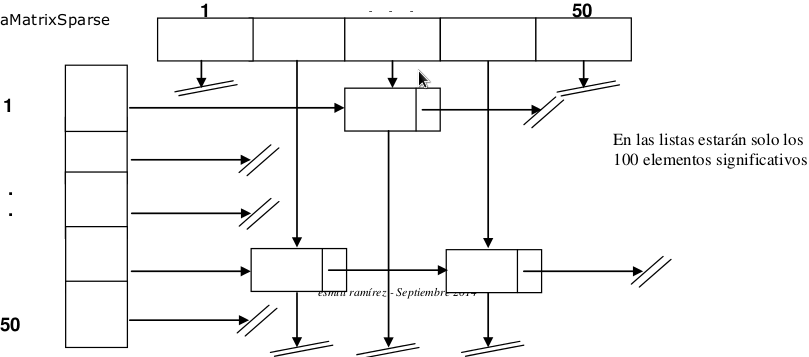
\includegraphics[width=0.85\textwidth]{images/sparse.png}
  \end{center}
  \caption{Ejemplo de representación de una matriz de $50 \times 50$ en una matriz esparcida.}
  \label{fig:sparse}
\end{figure}

Ahora, cada elemento de la lista (Node) está formado por dos identificadores del tipo Pointer y dos de tipo Integer, que indican la fila y columna asociada. Además, el arreglo solo contiene un apuntador al tipo Node, el cálculo de su complejidad queda como:
\begin{lstlisting}[upquote=true, language=pseudo]
CM(aMatrixSparse) = CM(Row) + CM(Col) + 100 * CM(Node)
CM(aMatrixSparse) = (2 * (50-1+1) * CM(Node*)) + 100 * (2*CM(Integer) + 2*CM(Node*))
CM(aMatrixSparse) = (2 * 50 * 1) + 100 * (2 + 2) = 500 palabras
\end{lstlisting}

De esta forma se tiene un ahorro en memoria respecto a la representación completa de una matriz $50 \times 50$ de: 
\begin{lstlisting}[upquote=true, language=pseudo]
CM(aMatrix) - CM(aMatrixSparse) = (2500 - 500) palabras = 2000 palabras. 
\end{lstlisting}

Esto indica que aMatrixSparse es solo una quinta parte de aMatrix en espacio en memoria.

%%%%%%%%%%%%%%%%%%%%%%%%%%%%%%
\subsubsection{Implementación}

La forma clásica de implementar una estructura Sparse Matrix es empleando apuntadores para la definición de los elementos que la conformará. A continuación se muestra una posible representación implementada con apuntadores.

\begin{lstlisting}[upquote=true, language=pseudo]
class Node <T>
public:
  T tInfo
  Integer iIdF, iIdC
  Node<T>* pNextR, pNextC
end

class NodeR <T>		// encabezados de las filas de la matriz
public:
  Integer iIdR
  T	tInfo
  NodeR <T>* pNext
  Node <T>* pFirst
end

class NodeC <T>		// encabezados de las columnas de la matriz
public:
  Integer iIdC
  NodeC <T>* pNext
  Node <T>* pFirst
end

class HeadNodeM <T>
public:
  NodeR <T>* pFirstR
  NodeC <T>* pFirstC
end

class SparseMatrix <T>
public:
  HeadNodeM <T>* Matrix
  function isElementOf (Integer iI, iJ) : Boolean
  void Insert (T tInfo, Integer iI, iJ)
  void Delete (Integer iI, iJ)
end
\end{lstlisting}

Nótese que las listas dentro de una matriz esparcida también se pueden usar doblemente enlazadas incorporando dos apuntadores a cada tipo Node: uno para el previo por fila y otro para el previo por columna (o en las listas de nodos cabeza (i.e. Node* pPrevR, pPrevC).


%%%%%%%%%%%%%%%%%%%%%%%%%%%%%%
\subsubsection{Ventajas y Desventajas}

Con una matriz esparcida se ahorra espacio en memoria cuando el número de nodos es muy pequeño respecto al número de elementos totales de la matriz. Se suele considerar un ahorro de memoria razonable cuando la cantidad de elementos significativos es un porcentaje de la cantidad total de nodos posibles (un aproximado que varía y puede llegar hasta un $20\%$ del total). Adicionalmente, con una representación basada en apuntadores es posible agregar/eliminar filas/columnas y nodos de forma sencilla.

En contraparte, cuando existen pocos elementos "no nulos" una solución basada en matriz esparcida puede no ser la más conveniente ya que ocupará más memoria que su contraparte estática a medida que el número de nodos sea mayor. En ese caso, se debe utilizar otra implementación que siga siendo dinámica pero que ocupe menos espacio en memoria (i.e. lista de adyacencia).

Por otro lado en implementaciones de matrices esparcidas, las operaciones de insertar y eliminar tienen un mayor nivel dificultad en su implementación y en su mayoría de complejidad $O(N)$ debido a las búsquedas lineales en una o varias listas.

%%%%%%%%%%%%%%%%%%%%%%%%%%%%%%%%%%%%%%%%%%%%%%%%%%%%%%%%
%%%%%%%%%%%%%%%%%%%%%%%%%%%%%%%%%%%%%%%%%%%%%%%%%%%%%%%%
\section{Tipo Stack}

Es una estructura de datos representado como un conjunto de elementos ordenados, donde el acceso a cada uno de sus elementos es en orden inverso a como se han agregado. El tipo Stack, sigue el esquema LIFO (\textit{last in first out}) donde el último en entrar (ser insertado en la estructura) será el primero en salir o ser tratado para almacenar y recuperar datos. Hay múltiples ámbitos donde se utilizan este tipo pila como estructura de datos debido su simplicidad y orden implícito. (e.g. la pila de ambientes de programas, simulación de una pila de libros o una mano de cartas, almacenar expresiones en notación polaca, etc.). En todo momento, solamente se tiene acceso a la parte superior de la pila (tope).  Para el manejo de los datos, las operaciones actúan sobre el tope de la pila: colocar un objeto (push/apilar) y su operación inversa, retirar el último elemento apilado (pop/desapilar).

La Fig. \ref{fig:stack1} se observa de forma gráfica un tipo Stack. Se puede ver que existe un tope y una base, donde los elementos entran a la pila por el tope y el primer elemento insertado siempre formará la base.

\begin{figure}[htp!]
  \begin{center}
    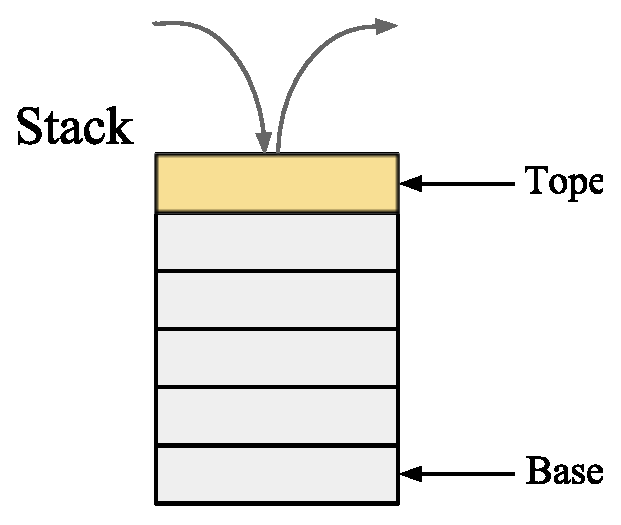
\includegraphics[width=0.35\textwidth]{images/stack.eps}
  \end{center}
  \caption{Representación gráfica del tipo Stack.}
  \label{fig:stack1}
\end{figure}

%%%%%%%%%%%%%%%%%%%%%%%%%%%%%%
\subsection{Especificación}

Dada la naturaleza del tipo Stack, la especificación de la clase resulta simple en cuanto a las funciones que emplea. A continuación se describe:

\begin{lstlisting}[upquote=true, language=pseudo]
class Stack <T>
public:
  Constructor Stack()	//construye la pila vacía.
  Destructor Stack()	//destruye la pila.
  function IsEmpty() : Boolean	//indica si la pila está vacía o no
  void Push(ref T x)	//agrega un nuevo elemento al tope de la pila. Ssegura que  Top()==x
  void Pop()	//precondición: la pila no puede estar vacía. Elimina el elemento del tope
  function Size() : Integer		//devuelve el \# de elementos en la pila
  function Top() : T	//precondición: la pila no puede estar vacía y retorna la información del tope
end
\end{lstlisting}

%%%%%%%%%%%%%%%%%%%%%%%%%%%%%%
\subsection{Implementación}

\paragraph{Implementación reutilizando la clase List}

Empleando el mecanismo de herencia, se puede implementar una pila basado en superclase lista aplicando todas las operaciones definidas en su especificación. Se emplea la herencia simple, donde todos los miembros públicos de la clase List serán privados dentro de la subclase Stack. 

\begin{lstlisting}[upquote=true, language=pseudo]
class Stack <T> inherited List <T>
public:
  Constructor Stack()	//construye la pila vacía. El const. de la superclase es invocada implícitamente
    //se puede invocar a this.List() pero no es necesario
  end

  Destructor Stack ()	//se destruye la pila. El destructor de la superclase es invocada implícitamente
  end

  function IsEmpty() : Boolean	//la pila está vacía si la lista (superclase) lo está
    return List<T>::IsEmpty()
  end

  void Push (ref T x)	// se asume que el tope es el primero de la lista
    Insert(x, First())
  end

  void Pop()		// dado que el tope es el primero de la lista, se elimina el primero
    Delete (First())
  end

  function Size() : Integer	//el tamaño de la pila se reduce a saber el tamaño de la lista
    return List<T>::Size()
  end

  function Top() : T	//retorna el elemento del tope, es decir, el 1ro de la lista
    return Get (*First())
  end
end
\end{lstlisting}

\paragraph{Implementación con apuntadores}

En esta caso, se realiza la implementación directamente con apuntadores al tipo Node siguiendo la especificación ya definida.

\begin{lstlisting}[upquote=true, language=pseudo]
class Node <T>
public:
  T tInfo
  Node<T>* pNext
end

class Stack <T>
private:
  Node<T>* pTop
  Integer iN

public:
  Constructor Stack()
    iN = 0
    pTop = NIL
  end

  Destructor Stack ()
    while pTop != NIL do
      Node<T>* pTemp = *pTop
      pTop = *pTop.pNext
      delete pTemp
	end
  end

  function IsEmpty() : Boolean
    return iN == 0
  end

  void Push (ref T x)
    Node<T>* pNew = new Node
    *pNew.x = *x
    *pNew.pNext = pTop
    pTop = pNew
    iN = iN + 1
  end

  void Pop()
    Node<T>* pTemp = pTop
    pTop = *pTop.pNext
    delete pTemp
    iN = iN - 1
  end

  function Size() : Integer
    return iN
  end

  function Top() : T
    return *pTop.tInfo
  end
end
\end{lstlisting}

%%%%%%%%%%%%%%%%%%%%%%%%%%%%%%
\subsection{Algoritmos}

A continuación una serie de algoritmos sencillos para demostrar el uso del tipo Stack.

\subsubsection{Paréntesis}

El problema de la paréntesis consiste en verificar que una secuencia de paréntesis sea correcta en al abrir-cerrar, es decir, se consideran correctos (()), [{}], {()[]} dado que para símbolo de paréntesis de apertura siempre tendrá su equivalente de cierre (basado en agrupamiento). Se consideran incorrectos los siguientes por ejemplo (()(, [[)]] ([)] entre otros.

\begin{lstlisting}[upquote=true, language=pseudo]
function Parenthesis(String strText, Integer iN) : Boolean
  Stack<Char> S
  for Integer iK = 1 to iN do
    if strText[ik] == '(' or strText[ik] == '[' or strText[ik] == '{' then
      S.Push(strText[ik])
    elseif S.IsEmpty() then
      return false
    else 	//verificar o no que sea ')', ']' o '}'
      S.Pop()
    end
  end
  return S.IsEmpty()
end
String strText = "{()()[]}"
if Parenthesis(strText, 8) then
  Print("Correcto")
end
\end{lstlisting}

La estructura de la pila garantiza que si no está vacía al final del algoritmo entonces no están colocados los paréntesis correctamente. Del mismo modo, si la pila llega a estar vacía antes de finalizar, entonces tampoco es incorrecto también.

\subsubsection{Notación PostFija}

La notación postfija o notación polaca inversa (\textit{Reverse Polish Notation} - RPN) es un método algebraico alternativo de representación de datos de entrada. En la RPN cada operador está antes de sus operandos, por ejemplo 3 4 + representa 3 + 4.

\begin{lstlisting}[upquote=true, language=pseudo]
function IsDigit(Char cValue) : Boolean
  return (cValue >= '0' and cValue <= '9')
end

function Char2Int(Char cValue) : Integer
  return cValue - '0'
end

function Compute(Integer iOp1, iOp2, Char cOp) : Integer
  if cOp == '+' then
    return iOp1 + iOp2
  elseif cOp == '-' then
    return iOp1 - iOp2
  elseif cOp == '*' then
    return iOp1 * iOp2
  elseif cOp == '/' then
    return iOp1 / iOp2		//iOp2 must be != 0
end


function RPN(String strExp, Integer iN) : Integer //Reverse Polish Notation
  Integer iOp1, iOp2
  Stack<Integer> S
  for Integer iK = 1 to iN do
    if IsDigit(strExp[iK]) then
      S.Push(Char2Int(strExp[iK]))
    else
      iOp1 = S.Top()
      S.Pop()
      iOp2 = S.Top()
      S.Pop()
      S.Push(Compute(iOp1, iOp2, strExp[iK]))
    end
  end
  return S.Top()
end

Print (RPN("59+2*", 5))		//output: 28
\end{lstlisting}

\subsubsection{Invertir Pila}

Utilizando únicamente las primitivas de la clase Stack, la idea es invertirla \textbf{sin utilizar} estructuras auxiliares. Este problema se basa en el hecho de aprovechar que las invocaciones recursivas se comportan como una pila de estados y permiten guardar en cada estado, una serie de variables.

\begin{lstlisting}[upquote=true, language=pseudo]
void InsertEnd(ref Stack<Integer> S, Integer iValue)
  if S.IsEmpty() then
    S.Push(iValue)
  else
    Integer iTop = S.Top()
    S.Pop()
    InsertEnd(ref S, iValue)
    S.Push(iTop)
  end
end

void Reverse(ref Stack<Integer> S)
  if not S.IsEmpty() then
    Integer iTop = S.Top()
    S.Pop()
    Reverse(ref S)
    InsertEnd(ref S, iTop)
  end
end

void PrintStack(Stack S)
  while not S.IsEmpty() do
    Print (S.Top())
    S.Pop()
  end
end

Stack<Integer> sValues
fillWithSomeValues (ref sValues)	//asignarle valores
PrintStack(sValues)		//i.e. 8 6 3 5 2 7 9
Reverse(ref sValues)
PrintStack(sValues)		//i.e. 9 7 2 5 3 6 8
\end{lstlisting}

%%%%%%%%%%%%%%%%%%%%%%%%%%%%%%
\subsection{Recursión} \label{sec:recstack}

Es posible emplear una estructura de pila para simular los ambientes de programas recursivos (recursión simple/ múltiple/ anidada/ indirecta). La idea consiste en apilar los resultados obtenidos en un ambiente, para luego combinarlos (extracción del tope) con una operación actual en cierto estado recursivo. De esta forma, es posible simular un algoritmo recursivo de forma iterativa empleando una pila para almacenar los resultados de cada ambiente “recursivo”.

Veamos un ejemplo simple con la función Factorial:

\textbf{Versión Iterativa}

Su versión clásica iterativa sirve como guía.

\begin{lstlisting}[upquote=true, language=pseudo]
function Factorial(Integer iN) : Integer
  Integer iResult = 0
  if iN <= 1 then
    return 1
  else
    iResult = Factorial (n - 1)
    return iResult * n
  end
end
\end{lstlisting}

\textbf{Versión que simula la recursión}

Una forma de simularla es añadiendo todos los valores y con los valores, ir extrayéndolos uno a uno y calcular el valor del factorial.

\begin{lstlisting}[upquote=true, language=pseudo]
function Factorial(Integer iN) : Integer
  Integer iResult = 1
  Stack <Integer> S
  while iN > 1 do
    S.Push(iN)
    iN = iN - 1
  end
  iResult = 1
  while (not S.IsEmpty()) do
    iResult =  iResult * S.Top()
    P.Pop()
  end
end
\end{lstlisting}

Otra forma de plantear la recursión con pila del mismo ejemplo es insertar solo el primer elemento antes de iniciar un ciclo en donde mientras no sea vacío calcular el valor deseado. Luego, si aún quedan datos por procesar, volver a apilar y se repite el proceso:

\begin{lstlisting}[upquote=true, language=pseudo]
function Factorial(Integer iN) : Integer
    Integer iResult = 1
    Stack <Integer> S
    S.Push(iN)
    iN = iN - 1
    while (not S.IsEmpty()) do
        iResult =  iResult * S.Top()
        S.Top()
        if (iN >= 1) then
            S.push(iN)
            iN =  iN - 1
        end
    end
    return iResult
end
\end{lstlisting}

%%%%%%%%%%%%%%%%%%%%%%%%%%%%%%%%%%%%%%%%%%%%%%%%%%%%%%%%
\section{Tipo Queue}

Es una estructura de datos representada como una lista ordenada donde el acceso a sus elementos se realiza desde un extremo de ésta. Una cola sigue el esquema FIFO (\textit{first in first out}) donde el primer elemento en ser agregado será el primero en ser removido o tratado para almacenar y recuperar datos. En una cola existe la definición de \textit{back} (por donde se insertan los elementos) y \textit{front} (por donde se extraen). El proceso de añadir un elemento se conoce como encolar (queue) y el proceso inverso desencolar (dequeue). En muchos problemas se utilizan colas: cola en una taquilla, cola de impresión, cola de transacciones bancarias en software, cola de autos, etc.

La Fig. \ref{fig:queue} muestra la forma del tipo Queue donde se aprecia el Back (por donde se insertan los elementos) y Front (por donde se extraen los elementos).

\begin{figure}[htp!]
  \begin{center}
    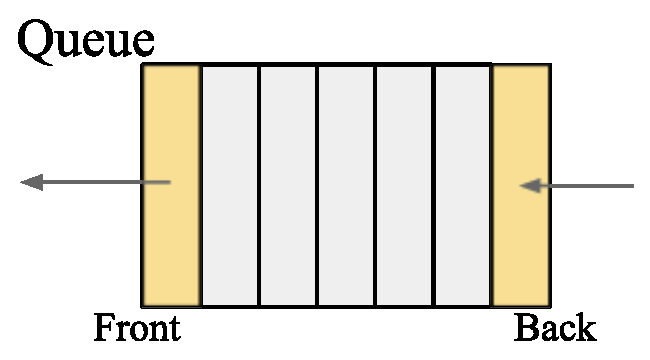
\includegraphics[width=0.35\textwidth]{images/queue.eps}
  \end{center}
  \caption{Representación gráfica del tipo Queue.}
  \label{fig:queue}
\end{figure}

%%%%%%%%%%%%%%%%%%%%%%%%%%%%%%%
\subsection{Especificación}

\begin{lstlisting}[upquote=true, language=pseudo]
class Queue <T>
public:
    Constructor Queue()	// construye la cola vacía
    Destructor Queue()	// destruye la cola

    function IsEmpty() : Boolean	// indica si la cola está vacía o no
    void Enqueue(ref T x)		// agrega el elemento x al final de la cola
    void Dequeue()		// precondición: cola no vacía, elimina el elemento que está primero en la cola
    function Size() : Integer		// devuelve el \# de elementos de la cola
    function Head() : T		// precondición: cola no vacía, retorna la información del primer elemento de la cola
end
\end{lstlisting}

La especificación del tipo Queue es muy simple y cuenta básicamente con las funciones de Enqueue, Dequeue y Head las cuales permiten que opere con el esquema FIFO.

%%%%%%%%%%%%%%%%%%%%%%%%%%%%%%%
\subsection{Implementación}

Al igual que la clase Stack, es posible implementar la clase Queue como una clase que hereda de List o con apuntadores simples.

\paragraph{Implementación reutilizando la clase List}

Empleando el mecanismo de herencia, se puede implementar una pila basado en superclase lista que implemente todas las operaciones del tipo Queue empleando herencia simple.

\begin{lstlisting}[upquote=true, language=pseudo]
class Queue <T> inherited List <T>
public:
  Constructor Queue()	// se construye la cola vacía. El constructor de la superclase es invocada implícitamente
  end

  Destructor Queue ()	// se destruye la cola. El destructor de la superclase es invocada implícitamente
  end

  function IsEmpty() : Boolean	// la cola está vacía si la lista (superclase) lo está
    return List<T>::IsEmpty()
  end

  void Enqueue (ref T x)	// se inserta el elemento al final de la cola
    Insert(x, Last())
  end

  void Dequeue()	// se elimina el que está de primero
    Delete (First())
  end

  function Size() : Integer	// el tamaño de la pila se reduce a saber el tamaño de la lista
    return List<T>::Size()
  end

  function Head() : T	// se accede al primer elemento de la cola (el elemento atendido)
    return Get (*First())
  end
end
\end{lstlisting}

\paragraph{Implementación con apuntadores}

En este caso, se realiza la implementación directamente con apuntadores al tipo Node.

\begin{lstlisting}[upquote=true, language=pseudo]
class Node <T>
public:
  T tInfo
  Node<T>* pNext
end

class Queue <T>
private:
  Node<T>* pFirst
  Node<T>* pLast
  Integer iN

public:
  Constructor Queue()
    iN = 0
    pFirst = pLast = NIL
  end

  Destructor Queue ()
    Node<T>* pTemp	
    while pFirst != NIL do
      pTemp =  pFirst
      pFirst =  *pFirst.pNext
      delete pTemp
    end
  end

  function IsEmpty() : Boolean
    return iN == 0
  end

  void Enqueue (ref T x)
    Node<T>* pNew = new Node
    *pNew.tInfo = *x
    *pNew.pNext = NULL
    if pFirst == NULL then
      pFirst = pNew
    else
      *pLast.pNext = pNew
    end
    pLast = pNew
    iN = iN + 1
  end

  void Dequeue()
    Node<T>* pTemp = pFirst
    pFirst =  *pFirst.pNext
    delete pTemp
    iN = iN - 1
    if pFirst == NULL then
      pLast = NULL
    end
  end

  function Size() : Integer
    return iN
  end

  function Head() : T
    return *pFirst.tInfo
  end
end
\end{lstlisting}

%%%%%%%%%%%%%%%%%%%%%%%%%%%%%%%%%%%%%%%%%%%%%%%%%%%%%%%%
\section{Otras estructuras}

Existen diversas estructuras de datos en la literatura para el uso en programas computacionales, a continuación se describen algunas de ellas.

%%%%%%%%%%%%%%%%%%%%%%%
\subsection{Tipo Double-ended Queue}

Una estructura de cola doblemente terminada, o abreviada como deque (double-ended queue) y a veces llamada lista enlazada cabeza-cola, es una generalización de cola donde los elementos pueden ser insertados o removidos por delante (head) o por detrás (tail). Esta estructura de datos puede contener restricciones en las operaciones de insertar/borrar. De hecho, la estructura cola y pila derivan de estas restricciones.

\begin{figure}[htp!]
  \begin{center}
    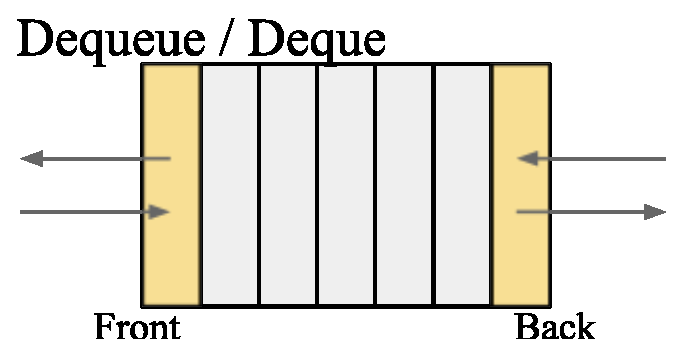
\includegraphics[width=0.35\textwidth]{images/deque.eps}
  \end{center}
  \caption{epresentación gráfica del tipo Deque.}
  \label{fig:deque}
\end{figure}

Las operaciones de la estructura deque son: insertar un elemento por detrás, insertar un elemento por delante, eliminar el último elemento, eliminar el primer elemento, extraer/procesar el primer/último elemento.

La implementación común de una estructura deque es empleando una arreglo dinámico (arrays deques) y una lista doblemente enlazada.

%%%%%%%%%%%%%%%%%%%%%%%
\subsection{Tipo Priority Queue}

Una cola de prioridad (\textit{priority queue}) es una estructura de datos muy similar a una lista pero cada elemento tiene una prioridad asociada. En una cola de prioridad, el elemento con más alta prioridad es manejado/procesado antes que un elemento de prioridad baja. Si existen dos elementos con prioridades iguales, entonces se procesa de acuerdo al orden de la cola.

Una implementación usual es con un heap (ver sección \ref{lb:heap}, parte VI) donde se permite extraer el elemento de mayor prioridad en $O(1)$.

%%%%%%%%%%%%%%%%%%%%%%%
\subsection{Tipo Associative Array}

Es una estructura de datos que almacena un par clave-valor (\textit{key-value}), donde la clave representa un identificador (generalmente único) y el valor consiste en el dato a almacenar. También se conoce como map, tabla de símbolos ó diccionario. Un arreglo asociativo se considera una colección donde siempre se añaden y remueven elementos del tipo clave-valor. Igualmente, es posible modificar el valor de un elemento de la colección dada la clave. Así, existe una forma de direccionamiento de una posición de la colección dada una clave (lookup).

Una implementación usual es con una tabla hash\footnote{Un hash table emplea una función de hash para calcular el índice dentro de un arreglo de buckets o slots desde donde puede ser ubicado/almacenado cada elemento.} ya que permite una correspondencia (\textit{mapping}) entre valores y claves.

La utilidad de estructuras de arreglos asociativos deriva básicamente en el almacenamiento de datos basados en operaciones de búsqueda, eliminación e inserción. Las operaciones comunes en este tipo de estructura son:
\begin{itemize}
\item Insert: Agrega un par (key, value) a la colección, realizando una asociación de la clave con su valor asociado. Los parámetros de está función son key y value.
\item Modify: Reemplaza el valor de uno de los pares (key,value) existentes en la colección, cambiando el valor almacenado en cierto key. Los parámetros de está función son key y value.
\item Delete: Elimina el valor de uno de los pares (key,value) existentes en la colección. Solo requiere el parámetro key.
\item Lookup: Busca el valor (si existe) que está asociado a cierto valor de key. El parámetro de está función es el valor de key y retorna value. Si no se encuentra un valor asociado, entonces deber retornar un valor que indique nulo (o una excepción).
\item Size: Retorna el número de elementos almacenados en la colección
\end{itemize}
Generalmente, la implementación en diversos lenguajes de programación de esta estructura de datos se conoce como map o hash. Un ejemplo de arreglos asociativos se puede observar en una empresa de alquiler de autos:
\begin{lstlisting}[upquote=true, language=html]
{"Ford BRD052" : "Luis Martinelli"}
{"Volkswagen AFV867" : "Luis Martinelli"}
{"Ford AAR309" : "Luisa Martinelli"}
\end{lstlisting}

Existe otra estructura de datos que representa una generalización del arreglo asociativo llamada multimap o multihash y permite que sea asociado más de un valor para una clave dada. 

%%%%%%%%%%%%%%%%%%%%%%%
\subsection{Tipo Set}

Un conjunto (set) es un tipo de dato que almacena valores sin un orden en particular sin repetición. Un set es la implementación matemática de un conjunto finito considerando sus operaciones (unión, intersección, diferencia y subconjunto). Del mismo modo, la estructura de datos conjunto puede ser estática (inmutable) o dinámica (mutable). La primera de éstas permite hacer consultas para un valor dado y determinar si pertenecen o no a un conjunto. La segunda permite las mismas operaciones que la estática añadiendo inserción y eliminación.

Un conjunto puede ser de cualquier tipo de dato e implementado de forma contigua en memoria (arreglos) o de forma dispersa (apuntadores). Las operaciones básicas de una estructura conjunto se pueden resumir en: isEmpty, size, insert, delete, add y elementOf.
Existe una estructura de datos llamada multiset o bag la cual es una generalización del tipo set. La diferencia radica en que permite repetir valores. De esta forma, es posible considerar dos elementos iguales como un solo elemento y manteniendo un contador de dicho elemento ó considerados equivalentes y almacenarlos de forma distinta y única. Dependiendo de la implementación de conjunto, se pueden establecer relaciones de equivalencia dentro de los conjuntos. 

%%%%%%%%%%%%%%%%%%%%%%%%%%%%%%%%%%%%%%%%%%%%%%%%%%%%%%%%
\section{Ideas Finales}

\begin{itemize}
\item La estructura dinámica ofrece una ventaja sobre las estructuras estáticas porque permite expandir o reducir en tiempo de ejecución el número y tamaño que ocupan sus elementos
\item Las operaciones que se realizan sobre los tipos de datos dinámicos resultan más complejos que su contraparte estática
\item Básicamente, el tipo List, Stack, Queue y sus derivados ofrecen un orden entre sus elementos tal que imponen restricciones de cómo acceder, insertar o eliminar dichos valores
\item De forma general, es posible implementar diversas estructuras de datos basados en el tipo List. Adicionalmente, el uso de apuntadores ofrece una flexibilidad que se puede adecuar al problema a resolver
\end{itemize}

%%%%%%%%%%%%%%%%%%%%%%%%%%%%%%%%%%%%%%%%%%%%%%%%%%%%%%%%
\section{Problemas}

\begin{enumerate}
\item Las listas enlazadas son por definición estructuras de datos homogéneas (es decir, todos sus nodos almacenan elementos del mismo tipo y estructura). ¿Eso es totalmente cierto?, es decir, ¿Sería posible tener una lista que almacene elementos diferentes en cada uno de sus nodos (tanto en tipo como en estructura)? Justifique su respuesta
\item Implemente una lista basada en arreglos que simule una lista circular de caracteres con $n$ posiciones y dados dos enteros $m$ e $i$, imprima $m$ valores a partir de la posición $i$. 
\item Dada un tipo Sparse Matrix $M$, elabore un algoritmo que imprima los elementos de la diagonal principal si estos están presentes
\item Dada una pila, se desea conocer el promedio de los elementos que ella almacena. Como restricción la pila puede ser recorrida una sola vez.
\item ¿Cuál sería la utilidad de una cola que contenga el método BeTheFirst, que permite colocar un elemento al inicio de la cola?
\item Una cola medieval se comporta como una cola ordinaria, con la única diferencia de que los elementos almacenados en ella se dividen en dos grupos: nobles y plebeyos. Dentro de cada grupo, los elementos deben ser atendidos en orden de llegada; pero siempre que haya nobles en la cola, estos deben ser atendidos antes que los plebeyos. Implemente una cola medieval heredando de una cola normal, pero sobrescribiendo el método Enqueue.
\item Diseñe un algoritmo que, dado el esquema de prelación de las materias de la carrera Computación y el código de una materia, imprima un listado con todas las asignaturas que tengan prelación a una materia dada, en orden cronológico
\end{enumerate}